\chapter{Protótipos estruturais}\label{cap:prototipos}

% --- INTRODUÇÃO  ---

A análise independente da precipitação total (Capítulo~\ref{cap:resultados_tp}) e do vento a 10 metros (Capítulo~\ref{cap:resultados_wind10}) mostra que ambas as variáveis apresentam mudanças estruturais ao longo do ciclo de vida ciclônico, em função da intensidade dinâmica do sistema.
No entanto, a análise separada não permite quantificar a diferenciação espacial conjunta entre o vento a 10 metros e a precipitação em um mesmo referencial.
Nesse sentido, propõe-se aqui o \textit{protótipo estrutural}, uma visualização que superpõe, no mesmo domínio centrado no sistema, os campos de densidade de probabilidade espacial (PDFe) e os padrões EOF dominantes de ambas as variáveis.

Cada protótipo combina quatro camadas de informação geométrica: (i) os contornos PDFe dos quantis 75 e 90 para precipitação (azul) e vento (vermelho), que mapeiam as zonas de maior concentração probabilística de máximos; (ii) as cargas positiva (sólida) e negativa (pontilhada) do primeiro modo EOF de ambas as variáveis (verde para precipitação, laranja para vento); e (iii) as coordenadas modais ($\Delta x$, $\Delta y$) de cada campo em relação ao centro do vórtice (0,0), representadas por estrelas.
O domínio de análise corresponde ao quadro de $20^{\circ} \times 20^{\circ}$ centrado no núcleo ciclônico, delimitado por uma máscara circular de raio $9{,}5^{\circ}$.
Apresentam-se duas versões: a População Global (Fig.~\ref{fig:prototipo_global}) e o subconjunto de ciclones de alta vorticidade p90 (Fig.~\ref{fig:prototipo_p90}), organizadas em uma matriz de $3 \times 4$ painéis (regiões $\times$ fases evolutivas).

Essa construção utiliza os padrões EOF1 univariados de vento e precipitação (Capítulos~\ref{cap:resultados_wind10} e \ref{cap:resultados_tp}), calculados separadamente, e não o modo conjunto MEOF1 (Capítulo~\ref{chap:meof}).
Optou-se por essa abordagem porque, em várias combinações de região, fase e população, o vento domina quase completamente o MEOF1 (Seção~\ref{sec:discusion_meof}).
Nesses casos, a carga de precipitação do modo conjunto nem sempre representa a variabilidade própria da precipitação.
Os EOF1 univariados não têm esse problema, e cada um possui seu próprio teste de significância e variância explicada, verificados em seu respectivo capítulo.
O custo dessa escolha é que a separação entre os centros de vento e de precipitação provém de duas decomposições independentes, portanto não está garantida por construção.
Essa separação tem um respaldo indireto na correlação significativa entre as componentes principais de ambos os campos durante a maturidade em p90 ($|r|$ entre $0.31$ e $0.45$, Seção~\ref{sec:meof_coherencia}).
Além disso, nessa mesma combinação, ambos os campos contribuem de forma comparável ao MEOF1 (Capítulo~\ref{chap:meof},
Tabela~\ref{tab:meof_bias_check}), de modo que a geometria resultante não depende de forma crítica de qual decomposição seja utilizada.


\section{População Global}\label{sec:prototipo_global}

\begin{figure}[H]
\centering
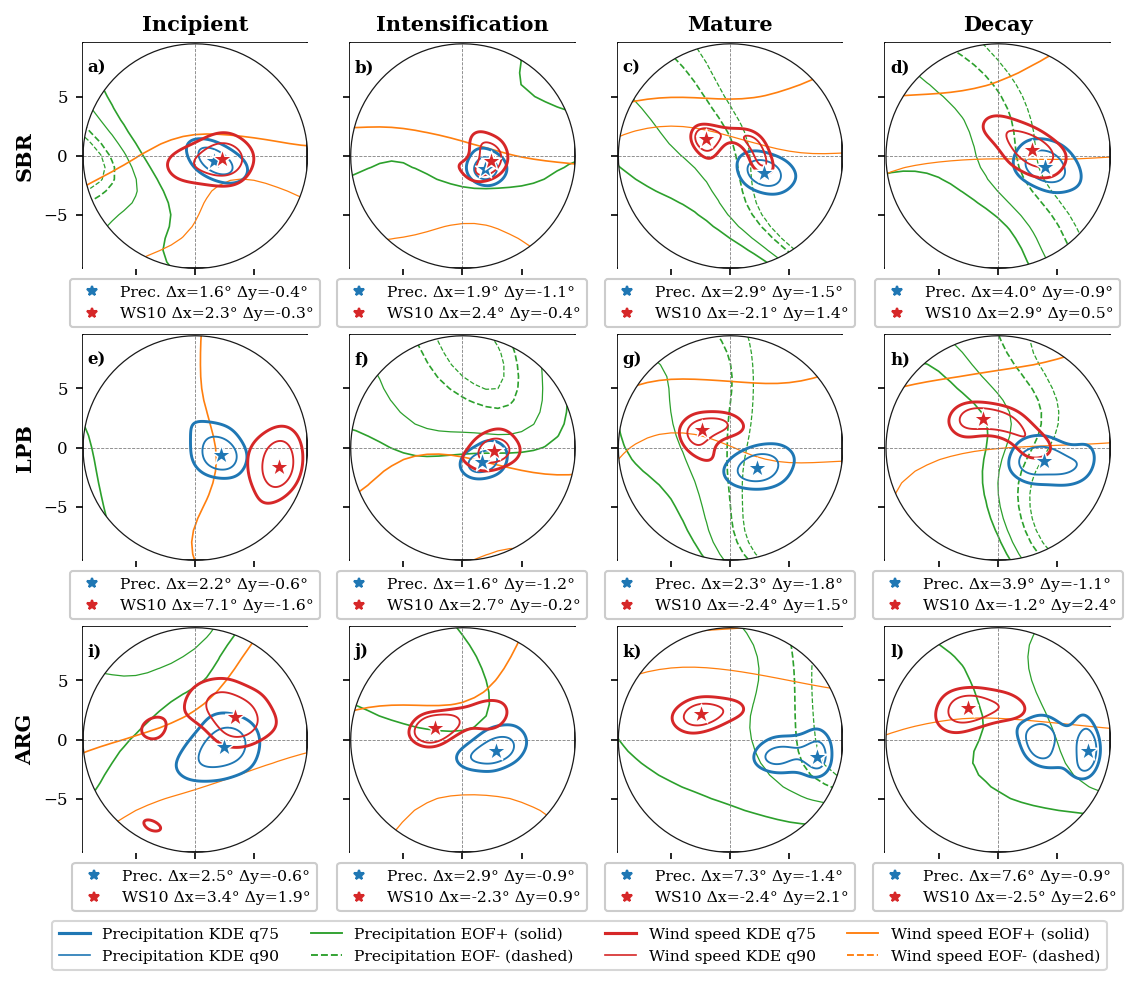
\includegraphics[width=\textwidth]{images/prototipos/prototipo_12panels_global.png}
\caption[Protótipos estruturais — População Global]{Protótipos estruturais para a População Global de ciclones extratropicais do Atlântico Sul-Ocidental. Cada painel superpõe, no domínio de $20^{\circ} \times 20^{\circ}$ centrado no sistema (0,0), os contornos PDFe dos quantis 75 e 90 de precipitação total (azul, linha grossa e fina respectivamente) e vento a 10 m (vermelho), juntamente com as cargas positivas (linha sólida) e negativas (linha pontilhada) do EOF1 de precipitação (verde) e vento (laranja). As estrelas azul e vermelha indicam as coordenadas modais ($\Delta x$, $\Delta y$) de cada campo. A matriz organiza as regiões de ciclogênese em linhas (SBR, LPB, ARG) e as fases evolutivas em colunas (Incipiente, Intensificação, Maturidade, Decaimento). A máscara circular delimita o domínio a um raio de $9{,}5^{\circ}$.}
\label{fig:prototipo_global}
\end{figure}

A Figura~\ref{fig:prototipo_global} apresenta os protótipos estruturais para a População Global, integrando a geometria probabilística dos máximos de ambas as variáveis com os padrões de maior variabilidade explicada (EOF1) para oferecer uma leitura simultânea da localização preferencial dos forçantes de precipitação e circulação ao longo do ciclo de vida.

Constrói-se a partir dos campos PDFe sobre a grade fixa centrada no sistema (Seção~\ref{subsec:kde_tp_global} para precipitação e Seção~\ref{sec:kde_espacial_global} para vento), combinados com o primeiro autovetor espacial das análises EOF independentes (Seção~\ref{sec:eof_tp} e Seção~\ref{sec:eof_wind10}). Os contornos de densidade são suavizados com um filtro gaussiano ($\sigma = 2$) antes de traçar os níveis dos quantis 75 e 90 segundo o critério de região de maior densidade (HDR). Seu propósito é sintetizar a coexistência ou diferenciação espacial entre circulação e precipitação nos ciclones ordinários, estabelecendo a linha de base em relação à qual será comparado o subconjunto de alta vorticidade na seção seguinte.

Durante as fases incipiente e intensificação (painéis a--f), os protótipos da População Global mostram uma colocalização relativa entre os máximos de precipitação e vento. Em SBR (painéis a--b), os contornos PDFe se superpõem parcialmente no quadrante oriental, com as modas de precipitação e vento separadas por apenas $0{,}1^{\circ}$--$0{,}7^{\circ}$ em latitude, enquanto as cargas do EOF1 de vento se estendem em direção ao noroeste. Em LPB (painéis e--f), tanto a precipitação quanto o vento se situam a leste-sudeste do centro durante a incipiência, com o vento sistematicamente mais afastado na componente zonal. A separação modal é de $4{,}9^{\circ}$ na fase incipiente (painel e) e se reduz a $1{,}1^{\circ}$ na intensificação (painel f). Em ARG (painéis i--j), o padrão já é bimodal desde as etapas iniciais. O PDFe de precipitação se mantém a leste-sudeste em ambas as fases, enquanto o de vento se desloca do nordeste (painel i) para o noroeste (painel j), antecipando a divergência que se consolida na maturidade. Essa colocalização parcial inicial reflete que, no regime médio, os forçantes frontais do WCB organizam ambos os campos no mesmo setor ativo do ciclone, antes que a diferenciação interna imponha geometrias distintas.

Ao transitar para a maturidade (painéis c, g, k) e o decaimento (painéis d, h, l), a arquitetura do protótipo se modifica de forma sistemática, ainda que moderada. Em LPB, os contornos PDFe de vento se deslocam em direção ao noroeste, coerentemente com a intensificação da circulação no flanco posterior do ciclone, enquanto os de precipitação se expandem em direção ao leste e sudeste, alcançando uma separação zonal de $4{,}7^{\circ}$ na maturidade (painel g) que se mantém em $5{,}1^{\circ}$ no decaimento (painel h). Em SBR, esse padrão é menos consistente. A separação zonal de $5{,}0^{\circ}$ observada na maturidade (painel c) se reduz a $1{,}1^{\circ}$ no decaimento (painel d), onde o vento retorna ao setor nordeste em vez de continuar se deslocando para o ocidente. No entanto, tanto os contornos PDFe quanto as cargas EOF1 mantêm, na População Global, uma extensão espacial considerável, sem que nenhum campo colapse para uma geometria estreita e bem definida, comportamento que reflete a heterogeneidade estrutural inerente ao catálogo completo, em que a integração de ciclones com diferentes taxas de oclusão, profundidades de vórtice e ambientes termodinâmicos dilui o sinal espacial de qualquer subconjunto estruturalmente coerente.

A comparação regional revela assimetrias na dinâmica de separação. Em ARG (painéis i--l), a divergência entre os PDFe de vento e precipitação é a mais pronunciada desde as fases iniciais, com a moda de vento deslocada para o noroeste ($\Delta x < 0$, $\Delta y > 0$) a partir da intensificação (painéis j--l), após iniciar a nordeste na fase incipiente (painel i, $\Delta x = 3{,}4^{\circ}$, $\Delta y = 1{,}9^{\circ}$), enquanto a moda de precipitação se mantém a leste-sudeste, com $\Delta x$ positivo e $\Delta y$ negativo nos quatro painéis. Esse comportamento contrasta com SBR e LPB, onde a separação meridional entre as modas é menor. Os contornos PDFe de precipitação de ARG, por sua vez, são os mais extensos das três regiões nas quatro fases. Essas diferenças regionais são coerentes com os padrões individuais descritos nos capítulos anteriores e confirmam que a síntese estrutural do protótipo não faz a média dessas diferenças, mas sim as preserva na leitura integrada.

\section{Subconjunto de alta vorticidade (p90)}\label{sec:prototipo_p90}

\begin{figure}[H]
\centering
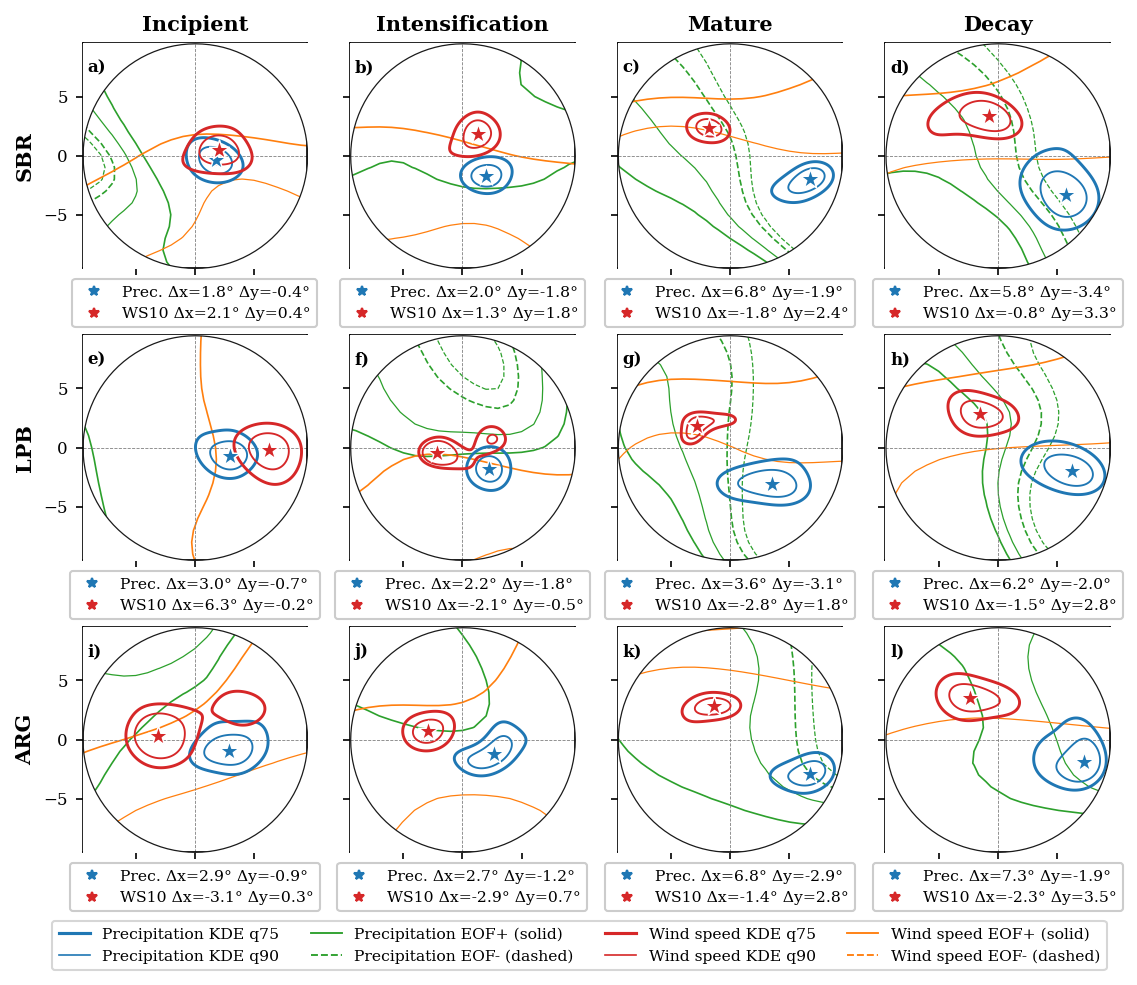
\includegraphics[width=\textwidth]{images/prototipos/prototipo_12panels_p90.png}
\caption[Protótipos estruturais — Subconjunto p90]{Protótipos estruturais para o subconjunto de ciclones de alta vorticidade (percentil 90 de vorticidade máxima). O formato dos painéis, a disposição matricial ($3 \times 4$, regiões $\times$ fases), a simbologia de cores e a escala do domínio centrado no sistema são idênticos aos da Figura~\ref{fig:prototipo_global}, permitindo quantificar diretamente a transformação estrutural que os sistemas p90 apresentam em relação à climatologia geral.}
\label{fig:prototipo_p90}
\end{figure}

A Figura~\ref{fig:prototipo_p90} apresenta os protótipos estruturais para o subconjunto de ciclones de alta vorticidade (p90), construídos com o mesmo procedimento metodológico da Figura~\ref{fig:prototipo_global}, mas restritos ao estrato de sistemas com vorticidade máxima no percentil 90. Essa visualização quantifica a diferenciação espacial entre circulação e precipitação nos sistemas p90 do Atlântico Sul-Ocidental, encerrando o argumento analítico desenvolvido nos capítulos de precipitação e vento. A comparação direta entre ambas as figuras, possível graças à escala, simbologia e disposição matricial idênticas, permite avaliar se a intensificação dinâmica amplifica ou reorganiza a disposição espacial relativa entre precipitação e vento.

O contraste visual com a População Global é imediato e profundo. Na fase de maturidade de SBR (painel c), o PDFe de precipitação (azul) entra em colapso em uma estrutura compacta deslocada para leste-sudeste ($\Delta x = 6{,}8^{\circ}$, $\Delta y = -1{,}9^{\circ}$), enquanto o PDFe de vento (vermelho) se concentra no quadrante noroeste ($\Delta x = -1{,}8^{\circ}$, $\Delta y = 2{,}4^{\circ}$). A separação entre ambas as modas é de ${\sim}9{,}5^{\circ}$ em distância euclidiana, em contraste com os ${\sim}5{,}8^{\circ}$ observados no mesmo painel (SBR, maturidade) da População Global. Essa diferença não é uniforme entre regiões e fases na População Global. Em SBR, a separação nas fases iniciais é mínima (painéis a-b, $0{,}7^{\circ}$--$0{,}9^{\circ}$), mas em LPB e ARG já se observam separações consideráveis mesmo na incipiência e na intensificação (até $5{,}5^{\circ}$ na intensificação de ARG, painel j), de modo que o contraste Global-vs-p90 é mais marcado em SBR do que nas outras duas regiões. Esse padrão de separação cruzada, precipitação a leste-sudeste, vento a noroeste, se reproduz com notória consistência em LPB (painéis g e h) e, com a maior magnitude das três regiões, em ARG (painéis k e l), onde a precipitação se desloca para leste ($\Delta x = 6{,}8^{\circ}$) e o vento mantém sua posição a noroeste ($\Delta x = -1{,}4^{\circ}$, $\Delta y = 2{,}8^{\circ}$), alcançando uma separação euclidiana próxima de $10^{\circ}$ na maturidade, que se amplia ainda mais no decaimento (painel l, ${\sim}11^{\circ}$), a maior de todo o subconjunto p90. Essa assinatura geométrica de quadrantes opostos constitui a expressão quantitativa da diferenciação espacial entre campos nos ciclones p90 da região.

A gênese dessa diferenciação nos sistemas de alta vorticidade poderia estar relacionada aos processos de oclusão documentados nas análises individuais de cada variável: a alta concentração do vento no quadrante noroeste, com densidades de até 27$\times10^{-4}$ em SBR e 23--25$\times10^{-4}$ em LPB (ARG se mantém mais baixa, ${\sim}19$--$21\times10^{-4}$; Seção~\ref{sec:kde_espacial_p90}), e a concentração do EOF1 de precipitação de até 36.5\% em LPB durante o decaimento (Seção~\ref{subsec:var_exp_tp}), são as duas faces quantitativas da mesma reorganização aqui sintetizada. O padrão de vento a noroeste é compatível com o ciclo de vida do tipo Shapiro-Keyser \citep{shapiro1990life}, no qual a cinta transportadora fria (\textit{cold conveyor belt}, CCB) se enrolaria em torno do núcleo do sistema em processo de oclusão, gerando o máximo de circulação de baixo nível no setor posterior do vórtice \citep{schemm2014linkage}. Simultaneamente, uma possível intrusão seca (\textit{dry intrusion}) proveniente da alta troposfera em direção ao núcleo do ciclone explicaria o espaço relativamente livre de precipitação que separa ambos os campos, embora esse mecanismo não seja medido diretamente em nenhum capítulo desta tese. O remanescente de umidade do WCB, por sua vez, é arrastado pela circulação ciclônica em direção à periferia, formando a estrutura em arco de precipitação no quadrante leste-sudeste, em uma posição mais próxima à do WCB do que à do quadrante ocluído que \citet{martin1999forcing} descreve para a banda enrolada (\textit{wrap-around precipitation}). A superposição desses dois processos, operando em quadrantes opostos, é o que gera a configuração diferenciada que o protótipo p90 capta.

A fase de decaimento (painéis d, h, l) mantém essa separação nas três regiões e a amplia em LPB e ARG. Em SBR (painel d), a moda de precipitação se desloca ainda mais para o sul ($\Delta x = 5{,}8^{\circ}$, $\Delta y = -3{,}4^{\circ}$) enquanto o vento migra para o norte ($\Delta x = -0{,}8^{\circ}$, $\Delta y = 3{,}3^{\circ}$), com uma separação euclidiana de ${\sim}9{,}3^{\circ}$, semelhante à da maturidade. Em LPB (painel h), os contornos PDFe de precipitação se estreitam em uma faixa arqueada em direção ao sul-sudeste, enquanto o vento mantém seu núcleo compacto a noroeste, com uma separação modal de $7{,}7^{\circ}$ na direção zonal. Esse comportamento reflete que, à medida que o ciclone se dissipa, a estrutura em arco mantém sua posição periférica mesmo quando a intensidade do sistema se debilita, enquanto o núcleo de vento se sustenta pela inércia ciclônica e pela advecção de vorticidade remanescente. As cargas do EOF1 de vento (laranja) mantêm sua orientação noroeste-sudoeste em todas as regiões durante o decaimento, enquanto as do EOF1 de precipitação (verde) adquirem uma curvatura arqueada para o sul, coerente com a geometria da faixa periférica documentada na Seção~\ref{subsec:eof1_tp_p90}.

As diferenças regionais na geometria da separação se manifestam primeiro na intensidade e extensão do campo de precipitação. Em SBR e LPB, a disponibilidade de umidade tropical canalizada pelo SALLJ \citep{reboita2026meteorology} poderia sustentar a estrutura em arco de precipitação com maior intensidade, aumentando a densidade no quadrante sudeste e ampliando a zona de alta probabilidade na maturidade e no decaimento. Em ARG (painéis i--l), a correlação entre o PC1 de precipitação e a vorticidade se mantém significativa durante todo o ciclo de vida em p90, incluindo a maturidade (Capítulo~\ref{cap:resultados_tp}), diferentemente de SBR e LPB, onde essa correlação deixa de ser significativa nessa fase, o que poderia explicar que a moda de precipitação mantenha, entre a maturidade e o decaimento, a posição mais estável das três regiões (deslocamento de ${\sim}1^{\circ}$, frente a ${\sim}1{,}7^{\circ}$ em SBR e ${\sim}2{,}9^{\circ}$ em LPB). No entanto, a separação euclidiana entre as modas de vento e precipitação não é menor do que em SBR e LPB, mas sim a maior das três regiões (${\sim}10$--$11^{\circ}$ na maturidade e no decaimento, contra ${\sim}9$--$9{,}5^{\circ}$ em SBR e ${\sim}8$--$9^{\circ}$ em LPB). A direção da diferenciação, precipitação a leste-sudeste, vento a noroeste, mantém-se sim consistente nas três regiões, revelando que a topologia fundamental da reorganização espacial é comum às três regiões, enquanto sua magnitude responde a uma combinação de fatores regionais que este capítulo não consegue atribuir de forma inequívoca ao regime de umidade oceânica.

A fase incipiente dos ciclones de alta vorticidade (painéis a, e, i) mostra que a diferenciação ainda não está plenamente desenvolvida, mas já exibe uma tendência diferenciada em relação à População Global equivalente. Em SBR (painel a), a moda de vento a nordeste ($\Delta x = 2{,}1^{\circ}$, $\Delta y = 0{,}4^{\circ}$) se separa levemente da moda de precipitação a leste ($\Delta x = 1{,}8^{\circ}$, $\Delta y = -0{,}4^{\circ}$), com os contornos PDFe ainda parcialmente superpostos, mas com centros diferenciados; a orientação para noroeste que caracterizará o vento em fases posteriores ainda não se manifesta nesta etapa incipiente. Em LPB (painel e), a separação zonal é mais notável desde o início ($\Delta x_{\text{vento}} = 6{,}3^{\circ}$, $\Delta x_{\text{prec}} = 3{,}0^{\circ}$), refletindo que os sistemas que eventualmente alcançarão o percentil 90 de vorticidade já exibem, durante sua gênese, uma assimetria frontal mais pronunciada do que a média, coerente com o maior gradiente térmico e o maior fluxo de umidade que caracteriza esses ambientes de ciclogênese mais ativos.

% SEÇÃO: DISCUSSÃO
\section{Discussão}\label{sec:discusion_prototipos}

% --- PARÁGRAFO 1: Validação da abordagem centrada no sistema e comparação com a literatura ---

A colocalização parcial documentada nos protótipos da População Global durante as fases incipiente e intensificação --consistente com o pico modal simultâneo de vento (12--15~m\,s$^{-1}$) e precipitação (10--20~mm/h) já relatado nessa mesma fase (Seções~\ref{sec:pdf_wind10} e~\ref{sec:pdf_tp})-- é coerente com os resultados de \citet{cardoso2022synoptic} para ciclones subtropicais do Atlântico Sul, uma estrutura geralmente distinta dos ETC baroclínicos catalogados nesta tese, que, por meio de um referencial lagrangiano semelhante, com um domínio de $20^{\circ} \times 20^{\circ}$ que acompanha o centro do ciclone, identificam anomalias positivas de vento a leste e nordeste da região ciclogenética RG1 e de precipitação a leste e dentro dela, calculadas pela média ao longo do ciclo de vida. Os protótipos do presente trabalho estendem esse resultado de duas maneiras: primeiro, ao incorporar explicitamente a fase evolutiva como eixo de estratificação, mostram que essa colocalização é própria das fases iniciais e não uma propriedade estática do ciclone; segundo, ao contrastar a População Global com o subconjunto p90, mostram que a colocalização se rompe de maneira quantificável nos sistemas p90. Essa distinção não pode ser inferida das análises climatológicas que calculam a média sobre o ciclo de vida completo \citep{gramcianinov2023impact}, e constitui o valor agregado central da abordagem de protótipos condicionais adotada nesta tese.

% --- PARÁGRAFO 2: A separação espacial em p90 e o modelo Shapiro-Keyser ---

A separação de quadrantes nos protótipos p90, vento a noroeste, precipitação a sudeste e sul, é compatível com a transição para o modelo de Shapiro-Keyser \citep{shapiro1990life}. Essa interpretação se apoia em um modelo conceitual geral, sem um estudo equivalente para o Atlântico Sul que confirme diretamente a sequência completa de oclusão nessa região.

% --- PARÁGRAFO 3: Comparação com estudos do Hemisfério Norte e transferibilidade do referencial conceitual ---

A arquitetura de quadrantes documentada nos protótipos p90 do Hemisfério Sul guarda certa correspondência, embora especulativa, com a organização do campo de vento relatada para ciclones explosivos do Hemisfério Norte. \citet{priestley2022improved} compõem os sistemas do percentil 90 de vorticidade ciclônica no ERA5 sobre um domínio de ${\sim}20^{\circ}$ centrado na trajetória, critério e escala comparáveis aos deste trabalho, e constatam que os ventos associados à CCB se concentram no flanco posterior-ocidental do vórtice; por inversão da circulação ciclônica entre hemisférios, essa posição é topologicamente análoga à concentração noroeste do vento documentada aqui. Cabe precisar que esse estudo não analisa o campo de precipitação, de modo que a comparação se limita estritamente ao vento. Isso sugere que a organização do vento em quadrantes opostos ao forçante do WCB é um traço compartilhado entre hemisférios, enquanto a geometria da estrutura em arco de precipitação do Atlântico Sul não tem um análogo conjunto vento-precipitação documentado na literatura do Hemisfério Norte consultada aqui.

% --- PARÁGRAFO 4: Os protótipos como ferramenta de diagnóstico: vínculo com o referencial multivariado ---

A abordagem de protótipos estruturais desenvolvida neste capítulo se alinha metodologicamente com propostas recentes que enfatizam a necessidade de vincular explicitamente a evolução dinâmica do sistema às suas manifestações estruturais. \citet{han2025system} propõem o \textit{SyCLoPS}, um referencial de classificação objetiva de alcance global que distingue dezesseis classes de sistemas de baixa pressão, incluindo os ciclones extratropicais como a classe mais frequente de seu catálogo. No entanto, seu referencial reserva a designação de sistemas de \textit{alto impacto}, e os composites de estrutura, precipitação e energia cinética associados a essa designação, aos ciclones tropicais, subtropicais e baixas polares, sem incluir os ciclones extratropicais nessa análise, apesar de serem a classe mais frequente de seu catálogo. Os protótipos apresentados neste capítulo abordam essa lacuna para o Atlântico Sul, quantificando, por meio de densidades de probabilidade espacial e modos dominantes de variabilidade (EOF), a posição relativa dos máximos de vento e precipitação em relação ao centro do vórtice, em um domínio centrado no sistema padronizado que permite a comparação direta entre regiões e fases do ciclo de vida. Essa abordagem revela, para os ciclones extratropicais da região, uma reorganização geométrica horizontal entre ambos os campos que um composite de corte vertical não capta diretamente. Essa combinação de geometria modal e densidade probabilística constitui, assim como o referencial proposto por \citet{corner2025classification} por meio de análise multivariada de parâmetros dinâmicos, um avanço em direção à caracterização objetiva e quantificada dos sistemas intensos ($\zeta_{850}$) no Atlântico Sul, uma região onde estudos equivalentes permaneceram, até agora, muito limitados.

% --- PARÁGRAFO 5: Limitações da abordagem e perspectivas futuras ---

Duas limitações da abordagem de protótipos merecem discussão explícita. Em primeiro lugar, a padronização do domínio centrado no sistema em uma grade fixa de $\pm 9{,}5^{\circ}$ implica que sistemas cuja estrutura em arco de precipitação se estende além desse raio, possível nos ciclones de maior escala horizontal, contribuem com densidade PDFe truncada nas bordas do domínio, subestimando a extensão real do campo de precipitação no protótipo. Essa limitação é inerente à abordagem composta centrada e foi reconhecida por \citet{cardoso2022synoptic}, que adotam explicitamente um domínio de $20^{\circ} \times 20^{\circ}$ precisamente para capturar os ventos extremos que podem ocorrer até 500 km do centro do ciclone. Em segundo lugar, a construção dos protótipos sobre o subconjunto estático p90 de vorticidade máxima implica que a amostra inclui sistemas em diferentes fases de seu ciclo de vida no momento de serem catalogados, embora a estratificação por fases mediante o algoritmo \textit{CycloPhaser} \citep{deSouza2025CycloPhaser} mitigue, em grande medida, esse efeito ao garantir que cada instante analisado pertença à fase correta do ciclone individual. Essas limitações abrem linhas de trabalho futuro: a extensão do domínio a $30^{\circ} \times 30^{\circ}$ para ciclones de grande escala, e a estratificação adicional pela velocidade de translação do sistema, um fator que, como apontam \citet{gramcianinov2023impact}, modula diretamente a duração do forçante e a extensão espacial dos campos dinâmicos, permitiriam refinar os protótipos em direção a representações mais completas da diversidade estrutural dos ciclones de alta vorticidade do Atlântico Sul.

\section{Síntese}\label{sec:sintesis_prototipos}

Os protótipos estruturais sintetizam, em uma representação geométrica única, a evolução diferencial da organização espacial dos campos de precipitação e vento associada aos ciclones extratropicais do Atlântico Sul-Ocidental ao longo de seu ciclo de vida. Na População Global, durante as fases incipiente e intensificação, as modas de precipitação e vento situam-se ambas no setor oriental em SBR e LPB, enquanto em ARG o vento já se desloca para noroeste na intensificação. Rumo à maturidade os campos se separam nas três regiões, embora em SBR a separação volte a diminuir no decaimento, e os contornos mantêm geometrias difusas que refletem a heterogeneidade da população geral.

Em contraste, o protótipo p90 revela uma reorganização qualitativa compatível com um processo de oclusão avançado. A superposição simultânea dos PDFe e EOF1 de ambas as variáveis no mesmo domínio quantifica a diferenciação espacial em sua expressão mais nítida. Os sistemas de alta vorticidade maduros e em decaimento apresentam os máximos de vento concentrados no quadrante noroeste, na zona onde a literatura situa a cinta transportadora fria, enquanto os máximos de precipitação ficam a leste-sudeste, na estrutura em arco. Em SBR e LPB, a separação entre modas na maturidade e no decaimento (${\sim}8$--$9{,}5^{\circ}$) supera claramente a da População Global (${\sim}2$--$6^{\circ}$). Em ARG, a separação é a maior das três regiões em p90 (${\sim}10$--$11^{\circ}$), mas é semelhante à de sua População Global, de modo que nessa região ela não é exclusiva dos sistemas mais intensos.

Do ponto de vista da dinâmica sinótica, esse resultado implica que os sistemas de alta vorticidade do Atlântico Sul não podem ser caracterizados pela colocalização simplificada de seus campos de precipitação e circulação. O centro de máxima variabilidade de precipitação e o centro de máxima variabilidade de vento operam em quadrantes opostos em relação ao centro do vórtice, com uma defasagem espacial que aumenta rumo à maturidade e ao decaimento. Em conclusão, os protótipos apresentados neste capítulo constituem a síntese espacial dos padrões dominantes de variabilidade de cada campo (EOF1 univariados) e de sua densidade de ocorrência (PDFe), consistente com dois resultados independentes dos capítulos anteriores. Primeiro, em p90-maturidade a vorticidade continua se correlacionando significativamente com a estrutura do vento nas três regiões ($|r|$ entre $0.26$ e $0.74$, Capítulo~\ref{cap:resultados_wind10}), enquanto para a precipitação essa correlação deixa de ser significativa em SBR e LPB ($|r|=0.17$ e $0.03$) e só se mantém em ARG ($|r|=0.24$, Capítulo~\ref{cap:resultados_tp}), o que sugere que a intensidade do vórtice deixa de prever a organização da precipitação com a mesma força com que continua prevendo a do vento. Segundo, a correlação entre as PC1 univariadas de precipitação e vento durante a maturidade em p90 é significativa nas três regiões ($|r|$ entre $0.31$ e $0.45$, Capítulo~\ref{chap:meof}), e sua relação com a localização real de cada EOF1 mostra que os eventos de um ciclo de vida que mais projetam sobre a estrutura em arco de precipitação tendem a ser os que menos projetam sobre o núcleo de vento. Essa separação de quadrantes é compatível com a reorganização do vórtice durante a oclusão, em que uma possível intrusão seca deslocaria a convecção para a periferia enquanto a cinta transportadora fria consolidaria a circulação de baixo nível no setor posterior.
